\documentclass{ltjbook}
\usepackage{docmute} 
\usepackage{../../myStyle} 

\begin{document}

\chapter{尤度と線形モデル}
\label{b24_linear_model}
前回は確率分布関数に含まれる変数の中で，パラメータの方が未知であると考えた尤度関数として捉え，尤度が最大になるようにパラメータの値を推定する\textbf{最尤推定法}について学びました。

今回はこれを，線形モデルに適用するお話です。線形モデルについては前期から今まで，折に触れては説明してきました。まず第\ref{ch07_Regression}講で回帰分析に触れ，続いて重回帰分析(第\ref{ch08_MultipleRegression}講)に進みました。後期に入ってからは，要因計画と仮説検定の合体技，\keytermL{分散分析}{ぶんさんぶんせき}の話になりましたが，そこでの推定方法は\keytermL{モーメント法}{もーめんとほう}，すなわち\keytermL{標本平均}{ひょうほんへいきん}や\keytermL{不偏分散}{ふへんぶんさん}を使ってのものでした。\keytermL{平方和}{へいほうわ}を\keytermL{自由度}{じゆうど}で割って，\keytermL{平均平方}{へいきんへいほう}を出し，その比が\keytermL{F分布}{Fぶんぷ}に従う，という考え方は，平均や分散から母数を考えようという発想と同じものだと言えます。

それに対して，前回は尤度から母数を考えようという発想でした。推定値は同じになるのですが，考え方が違っていることに注意して，線形モデルの最尤推定について考えていきます。

\section{回帰モデルの確率表現}
改めて線形モデル，とくに\keytermLsub{単回帰分析}{たんかいきぶんせき}{回帰分析}{かいきぶんせき}のモデルを復習しておきましょう。

データの組，$x_i,y_i$があったときに，変数$x$をつかって$y$を予測する，線形モデルを当てはめるということを考えるのでした。線形モデルは最も単純な一次式で，
\begin{align}
\hat{y}_i = \beta_0 + \beta_1 x_i
\end{align}
とし，予測値$\hat{y}$に誤差$\varepsilon$がついて実現値$y$が得られると考えて，
\begin{align}
y_i= \beta_0 + \beta_1 x_i + \varepsilon_i
\end{align}
とするのでした。第\ref{ch07_Regression}講でやった\keytermL{最小二乗法}{さいしょうにじょうほう}は，この式をデータに当てはめ，データの中で誤差が一番小さくなるように切片を求める，という方法だったことを思い出してください。あくまでも手元のデータの話しかしていませんでしたが，これに推測統計学のエッセンス，つまり手元のデータは標本に過ぎず，母集団の中でどうか，ということを考えたいと思います。

ところで，この時も仮定として誤差の分布に\keytermL{正規分布}{せいきぶんぷ}を仮定していましたね。誤差はさまざまな未知なる要因の積み重ねですから，数字を増やす方向に加わるのか，減らす方向に加わるのかは分かりません。それでも極端に大きな誤差というのは出にくく，平均周りの誤差が出やすいと考えるなら，単峰で左右対称のベルカーブのような形になるはずです。また，今回ここで考えているのは\keytermL{偶然誤差}{ぐうぜんごさ}ですから\footnote{これに対して\keytermL{系統誤差}{けいとうごさ}というのがありました。システマチックな誤差，という意味で，常に定数が加わるようなイメージです。体重計などの秤で何も測っていないときに目盛がずれているようなものですから，今回のケースではその補正には触れません。測定する際に気をつけるべきことで，気をつけてもなくならないのが偶然誤差です。}，その平均はゼロだと考えられます。ですから，$\varepsilon_i = y_i - \hat{y}_i$をデータ全体で最小にするようにモデルをフィッティングするのでした。ここまでは前期の復習になります。

\subsection{確率モデルとしての表現}
この線形モデルを確率モデルと考えて，最尤推定したい，というのがここでの狙いです。

\keytermLsub{最尤推定}{さいゆうすいてい}{最尤法}{さいゆうほう}をするためには，この回帰分析の式を確率モデルで表現しなければなりません。先ほどのモデル式の中に出てくる記号のなかで，確率的に変わるのは何かと言われれば，誤差$\varepsilon$です。
そしてこれは，正規分布に従うだろうと考えるのが自然なのでした。式で書くと，
\begin{align}
\varepsilon_i \sim N(0,\sigma)
\end{align}
ということになります。ここで誤差の平均が0である，ということを再確認してください。また，平均は0ですが，誤差は一定の幅で散らばって出てきますので，これを標準偏差$\sigma$で表しています。

さて，誤差が確率的に求まることがわかりましたが，$x$と$\hat{y}$の関係は確率的ではありません。切片や傾きは未知数ですが(母集団での切片と傾きのことになるので$\beta_0,\beta_1$と表記しますが)，これがわかりさえすれば$\hat{y}_i$と$x_i$の関係は確定的です。つまり，「確率分布に従う」を表す$\sim$という記号ではなく，「左辺はこのようになって\textbf{いる}」ということを記述するために，$=$を使って書くことができます。
\begin{align}
\hat{y}_i = \beta_0 + \beta_1 x_i
\end{align}
これが線形モデルです。誤差に邪魔されることがない，理想的な予測値$\hat{y}$は，$x_i$の一次関数の形で記述できる，ということです。実際のデータ$y_i$は$\hat{y}$に誤差がついて出てくるものですから，
\begin{align}
y_i = \hat{y}_i + \varepsilon_i
\end{align}
と書くことができます。

さて，これらを組み合わせていきましょう。最後の式から$\hat{y}$を消去する(線形モデルで代入する)と，
\begin{align}
y_i =  \beta_0 + \beta_1 x_i+ \varepsilon_i
\end{align}
ということになります。ここで$ \beta_0 + \beta_1 x_i$のところは確率的に変わるものではない，ということを思い出してください。

\begin{align}
y_i =
	\tcboxmath[
		enhanced,         % これは必須
		frame hidden,     % 枠を消す. これも enhanced 必須
		colback=cyan!10,
		overlay={
				\node[below,blue] at (frame.south) {確率的でないところ};
			}
	]{
		\beta_0 \quad +\quad \beta_1 x_i
	}
	+
	\tcboxmath[
		enhanced,         % これは必須
		frame hidden,     % 枠を消す. これも enhanced 必須
		colback=red!10,
		overlay={
				\node[below,red] at (frame.south) {確率的};
			}
	]{
		\varepsilon_i
	}
\end{align}

\vspace{0.5cm}
誤差$\varepsilon_i$は平均0を中心に確率的に散らばりますが，その前のところは確率的ではありませんので，これを組み合わせた式全体としては，最後に確率的な散らばりがひっついているような形になります。数式ではありませんが，イメージでいうとこんな感じ。
\begin{center}
	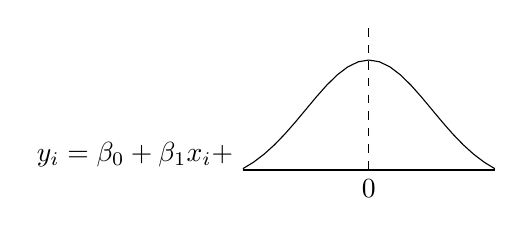
\begin{tikzpicture}[xscale = 0.8, yscale = 4]
		\coordinate (A) at (-2,0);
		\draw (A) node[left] {$y_i = \beta_0 + \beta_1 x_i + $};
		\draw [domain=-2:2] plot(\x, {exp((-(\x)^2)/2)/(sqrt(2*pi))-0.1});
		\draw [dashed] (0,0.4)--(0,-0.05);
		\draw (-2,-0.05)--(2,-0.05);
		\node (zero) at (0,-0.05)[below]{$0$};
	\end{tikzpicture}
\end{center}

さて，この「確率的でないところ」が確率分布の中に入り込むとしたら，誤差$\varepsilon_i$の平均値を一定の量，$\beta_0 + \beta_1 x_i$分だけ動かすことになります。
回帰直線が表しているのは，誤差のない予測の線でもあります。実際のデータはそれに誤差が伴って生じます。確率モデルになった線形モデルは，図\ref{fig:24_01}のようなイメージで考えるといいかもしれません。
\begin{figure}[ht]
	\centering
	\caption{予測直線にまとわりつく誤差}
	\label{fig:24_01}
	\includegraphics[keepaspectratio,width=0.8\linewidth]{figures/24_linear_model/linear_error.png}
\end{figure}

ここで正規分布がもつ2つのパラメータ，$\mu$と$\sigma$は，それぞれ\textbf{位置}と\textbf{幅}を表しているわけですが，確率的でないところはこの位置をズラすような作用をすることになります。

大事なところなので，もう一度式で確認しながら説明します。まず今回のモデルに含まれる情報は次のとおりです。
\begin{eqnarray}
	\hat{y}_i = \beta_0 + \beta_1 x_i \label{eq24_01}\\
	y_i = \hat{y}_i + \varepsilon_i \label{eq24_02}\\
	\varepsilon_i \sim N(0,\sigma)\label{eq24_03}
\end{eqnarray}
ここで式\ref{eq24_01}と\ref{eq24_02}を合わせて，
\begin{equation}
	\begin{array}{ccc}
		y_i & =    & \beta_0 + \beta_1 x_i +\varepsilon_i \\
		\varepsilon_i & \sim & N(0,\sigma)
	\end{array}
	\label{eq24_04}
\end{equation}
とします。ここで$\varepsilon_i$の中心は$0$で，それに$\beta_0 + \beta_1 x_i$が加わるのですから，
\begin{align}
y_i \sim N(\beta_0 + \beta_1 x_i, \sigma)
\end{align}
ということになります。

あるいは，式\ref{eq24_02}と\ref{eq24_03}から先に，
\begin{eqnarray}
	\hat{y}_i &=& \beta_0 + \beta_1 x_i \label{eq24_05}\\
	y_i &\sim& N(\hat{y}_i,\sigma) \label{eq24_06}
\end{eqnarray}
と考えて，この式\ref{eq24_06}の$\hat{y}_i$に式\ref{eq24_05}を代入しても，
\begin{align}
y_i \sim N(\beta_0 + \beta_1x_i, \sigma)
\end{align}
が得られます。どちらのルートでも結構ですから，自分のわかりやすい方で理解してください。一連の流れを図\ref{fig:24_02}にまとめてみました。
\begin{figure}[ht]
	\centering
	\caption{確率モデルと予測モデルの合体}
	\label{fig:24_02}
	\begin{tikzpicture}
		\coordinate (A) at (1,1);
		\coordinate (B) at (2,2);
		\coordinate (C) at (5,2);
		\coordinate (D) at (7,1);
		\coordinate (E) at (1,3);
		\coordinate (F) at (7,3);
		\coordinate (G) at (1,5);
		\coordinate (H) at (7,5);
		\coordinate (I) at (1,7);
		\coordinate (J) at (2.5,6.5);
		\coordinate (K) at (5,6.5);
		\coordinate (L) at (7,7);
		\draw[->] (B)--(C);
		\draw[->] (G)--(E);
		\draw[->] (H)--(F);
		\draw[->] (J)--(K);
		\node (I1) at (0.3,6.5) {$\hat{y}_i  = \beta_0 + \beta_1x_i \ldots$(1)};
		\node (I2) at (0.54,6)  {${y}_i  = \hat{y}_i + \varepsilon_i \ldots$(2)};
		\node (I3) at (0.5,5.5)  {$\varepsilon_i \sim N(0,\sigma) \ldots$(3)};
		\node (L1) at (7,6)  {$\varepsilon_i \sim N(0,\sigma)$};
		\node (L2) at (7,6.5) {${y}_i  = \beta_0 + \beta_1x_i + \varepsilon_i$};
		\node (A1) at (0.5,2.5) {$\hat{y}_i  = \beta_0 + \beta_1x_i$};
		\node (A2) at (0.5,2) {$y_i \sim N(\hat{y}_i,\sigma)$};
		\node (D1) at (7,2) {$y_i \sim N(\beta_0 + \beta_1 x_i,\sigma)$};
		\node (P1) at (3.5,6.5)[above] {(2)に(1)を代入};
		\node (P2) at (1,4)[left] {(2)に(3)を代入};
		\node (P3) at (7,4)[right] {};
		\node (P4) at (3.5,2)[below] {};
	\end{tikzpicture}
	
\end{figure}


これが回帰分析の\keytermL{確率モデル}{かくりつもでる}になります。
ポイントは，確率分布の位置を表すパラメータに，数式で表現された\textbf{構造}を書き込んだところにあります。狭義の\textbf{モデリング}とは，確率分布のパラメータに構造を与えるもの，ということができるでしょう。
この枠組みをさらに一般化すると，正規分布以外の確率分布にも線形モデルを適用できるようになります。これについては本章の後半で改めて説明します。

\section{回帰分析の最尤推定}

このようにして確率モデルを書くことができれば，あとはこれにしたがって「データがこの確率モデルから出てくる尤もらしさが最も高くなるように，未知パラメータを推定すれば良い」ということになります。
改めて確認ですが，今回のモデル$y_i \sim N(\beta_0 + \beta_1x_i, \sigma)$において未知な数字は$\beta_0,\beta_1,\sigma$の3つになります。


正規分布の式をちゃんと書くと，$x$という値が出てくる確率密度は
\begin{align}
p(x) = \frac{1}{\sqrt{2\pi \sigma^2}}exp\left( - \frac{(x-\mu)^2}{2\sigma^2}\right)
\end{align}
となります。この平均$\mu$のところに$\beta_0 + \beta_1 x_i$という数式を入れることになります。

すでに入り組んだ形をしているので，イメージしづらいところがあるかもしれませんが，あるデータ$y_i$が得られる確率密度は
\begin{align}
p(y_i) = \frac{1}{\sqrt{2\pi \sigma^2}}exp\left( -\frac{(y_i-\mu)^2}{2\sigma^2}\right)
\end{align}
ですから，$\mu=\hat{y_i} = \beta_0 + \beta_1 x_i$を代入して
\begin{align}
p(y_i) = \frac{1}{\sqrt{2\pi \sigma^2}}exp\left( -\frac{(y_i-\beta_0 - \beta_1 x_i)^2}{2\sigma^2}\right)
\end{align}
となります。

データは$i = 1,2,\cdots,N$とあり，それらが同じ母集団から独立に得られている，と考えます(i.i.d.)。つまり手元に同時にこれらのデータが出揃うときの尤度$L$は，上記の確率密度($p(y_i)$)を全部掛け合わせたもの\footnote{コインが表，表，裏，と出たら$\theta \times \theta \times (1-\theta)$と書けたことを思い出して！}，と考えることができますね。
$i$を$1$から$n$まで足し合わせることを総和する，といって$x_1+x_2+\cdots+x_N=\sum_{i=1}^N x_i$と表しますが，同様にすべて掛け合わせる総積は，
\begin{align}
x_1 \times x_2 \times \cdots x_N = \prod_{i=1}^N x_i
\end{align}
と書きます。ここでの記号$\prod$は\ruby{総積}{プロダクト}と言いますが，これを使って尤度$L(y_i)$を表現すると，次のようになります。

\begin{align}
L(y_i | \beta_0,\beta_1,\sigma) = \prod_{i=1}^N \frac{1}{\sqrt{2\pi \sigma^2}}exp\left(- \frac{(y_i-\beta_0 - \beta_1 x_i)^2}{2\sigma^2}\right)
\end{align}

ここで$L(y_i | \beta_0,\beta_1,\sigma) $という書き方の，$\mid$は何かというと，この縦線の右側にある$\beta_0,\beta_1,\sigma$が与えられた場合の，という条件つき確率の書き方を借りた\keyterm{尤度}{ゆうど}{likelihood}を表しています。

さてこれは確率(密度)の掛け算になりますから，すごく小さな数字になって実際の計算は大変です。そこで前回習ったように，尤度そのものではなく\keyterm{対数尤度}{たいすうゆうど}{log-likelihood}をとって，その最大値を求めるということにしたいと思います。対数をとると掛け算は足し算に変わりますから，$\prod \to \sum$に記号が変わりまして，対数尤度の関数は次のようになります。
\begin{align}
\log L(y_i | \beta_0,\beta_1,\sigma) = \sum_{i=1}^N \log \left[ \frac{1}{\sqrt{2\pi \sigma^2}}\exp\left(- \frac{(y_i-\beta_0 - \beta_1 x_i)^2}{2\sigma^2}\right) \right]
\end{align}

非常に面倒な形をしていますね！しかもこれは$\beta_0,\beta_1,\sigma$という3つの変数が同時に関わりますから，連立微分方程式を解くことになります。

ここからは少しテクい話になりますが，この式を展開していきましょう。$\frac{1}{\sqrt{2\pi\sigma^2}}=(2\pi\sigma^2)^{-1/2}$であることに注意して対数尤度を書き直すと，

\begin{align*}
\log L &= \log\prod_{i=1}^n (2\pi\sigma^2)^{-1/2}\exp\left(-\frac{(y_i-(\beta_0+\beta_1x_i))^2}{2\sigma^2}\right) \\
&= \sum_{i=1}^n \log\left[(2\pi\sigma^2)^{-1/2}\exp\left(-\frac{(y_i-(\beta_0+\beta_1x_i))^2}{2\sigma^2}\right)\right] \\
&= \sum_{i=1}^n \left[\log(2\pi\sigma^2)^{-1/2} + \log\exp\left(-\frac{(y_i-(\beta_0+\beta_1x_i))^2}{2\sigma^2}\right)\right] \\
&= \sum_{i=1}^n \left[-\frac{1}{2}\log(2\pi\sigma^2) - \frac{(y_i-(\beta_0+\beta_1x_i))^2}{2\sigma^2}\right]\\
&= \sum_{i=1}^n \left[-\frac{1}{2}\log(2\pi) - \frac{1}{2}\log(\sigma^2) - \frac{(y_i-(\beta_0+\beta_1x_i))^2}{2\sigma^2}\right]\\
&= -\frac{n}{2} \log(2\pi) - \frac{n}{2} \log(\sigma^2) - \frac{1}{2\sigma^2} \sum_{i=1}^{n} (y_i-(\beta_0+\beta_1x_i))^2
\end{align*}

こうしてみると，$\frac{n}{2} \log(2\pi)$は定数ですし，$\frac{n}{2} \log(\sigma^2) $は推定すべきパラメータ$\sigma^2$で，データによって変わるところではありません。
第3項の$\sum_{i=1}^{n} (y_i-(\beta_0+\beta_1x_i))^2$がデータによって変わるところで，これを最小化することを考える必要がありますが，これは最小二乗法で考えるべきポイントと同じですね。ですから，この最尤推定の結果得られる$\beta_0,\beta_1$の値は，\underline{最小二乗法の結果と一致}します。

もちろんこの面倒な計算は，Rがやってくれますから私たちはなんの心配もする必要はありません。
ですから，実質的にはただの回帰分析をすれば良いのです。

\subsection{実践例}
数字としてはなんら変わるところはないのですが，復習も兼ねて第\ref{ch09_Regression_onR}講でやった回帰分析をもう一度見てみましょう。
回帰分析の関数は\verb|lm|という関数名で，Rがデフォルトで持っている関数なのでした。実はこの関数，最尤推定値を返す関数だったのです。
そのときは\keytermL{最小二乗法}{さいしょうにじょうほう}の説明しかしていなかったのですが，関数の使い勝手のこともあって，最尤推定する関数でご紹介しておりました。
本当の意味で，最小二乗法のアルゴリズムで回帰分析をするときは\verb|lsfit|関数というものを使います。

使用例をコード\ref{code:24_01}に示しました。ここでは野球選手のデータを使って，身長から体重を予測するというモデルを実行しています\footnote{第\ref{ch09_Regression_onR}講と同じ分析結果です。}。データの\verb|batter|は，第\ref{ch09_Regression_onR}講の\texttt{code:\ref{code:09_01}}と\texttt{code:\ref{code:09_02}}で作ったものです。新しいスクリプトで始める場合は，先にこの2つを実行して\verb|batter|を作っておいてください。
\begin{lstlisting}[language=c++,label={code:24_01},caption={二つの推定法の比較}]
# 最小二乗法の推定
result.LS <- lsfit(x = batter$height, y = batter$weight)
result.LS$coefficients
# 最尤推定
result.LM <- lm(weight ~ height, data = batter)
summary(result.LM)
\end{lstlisting}
結果は出力\ref{RS:out24_01}のようになります。
\begin{Rscreen}{比較した結果}{out24_01}
	\begin{verbatim}
> # 最小二乗法の推定
> result.LS <- lsfit(x = batter$height, y = batter$weight)
> result.LS$coefficients
  Intercept           X 
-124.917552    1.166698 
> # 最尤推定
> result.LM <- lm(weight ~ height, data = batter)
> summary(result.LM)

Call:
lm(formula = weight ~ height, data = batter)

Residuals:
     Min       1Q   Median       3Q      Max 
-20.9217  -4.9213  -0.4214   4.0783  28.9118 

Coefficients:
              Estimate Std. Error t value Pr(>|t|)    
(Intercept) -124.91755   13.89317  -8.991   <2e-16 ***
height         1.16670    0.07746  15.063   <2e-16 ***
---
Signif. codes:  0 ‘***’ 0.001 ‘**’ 0.01 ‘*’ 0.05 ‘.’ 0.1 ‘ ’ 1

Residual standard error: 7.435 on 327 degrees of freedom
Multiple R-squared:  0.4096,	Adjusted R-squared:  0.4078 
F-statistic: 226.9 on 1 and 327 DF,  p-value: < 2.2e-16
    \end{verbatim}
\end{Rscreen}

これを見ると明らかなように，どちらの方法でやっても同じ推定値(切片$\beta_0=-124.918$，傾き$\beta_1=1.167$)になっていますね。また少し余談ではありますが，最尤推定した結果の最終行を見ると，$F$統計量が自由度$F(1,327)=226.9$とあり，この$p$値も計算されています。ここで線形モデルと要因計画・帰無仮説検定も関連があることがわかります\footnote{ここでは切片以外のすべての説明変数(今回の例では単回帰なので説明変数は一つですが)の傾きが0である，という帰無仮説にたいして検定が行われています。}。

方法が違っても推定値が同じ，というのは前回もお話ししたように，同じ母数を推定しているわけですからむしろ当然の結果です。1つの山の頂上に達するのに，複数のルートがあってもゴールは同じ，ということです。
違う点があるとすれば，最尤推定の場合は誤差の標準偏差$\sigma$も推定されているというところでしょうか。結果に$\sigma=...$という記載はありませんが，よく見ると\verb|Residuals|のところに残差$e$の最小値，最大値，四分位偏差，中央値などが示されており，誤差が分布するものと考えられていることがわかります。

今回は説明変数が1つの単回帰分析でしたが，説明変数の数が増えた\keytermsub{重回帰分析}{じゅうかいきぶんせき}{multiple regression analysis}{回帰分析}{かいきぶんせき}でも同じで，\verb|lm|関数はデータが正規分布から得られたものとした上で，尤度を最大にする推定値を返してくれます。

Rで回帰分析をしたついでに，この結果をplot関数にいれてみましょう。
\begin{lstlisting}[language=c++,label={code:24_02},caption={回帰分析の結果オブジェクトをプロットに入れる}]
	par(mfrow = c(2, 2)) # 2x2の配置にする
	plot(result.LM)	
\end{lstlisting}

4つの図が表示されますが，ここでは$2\times 2$の配置にしています。出力されるのは図\ref{fig:24_03}のようになります。
\begin{figure}[ht]
	\centering
	\caption{回帰分析の結果をプロットすると4枚の図が出てくる}
	\label{fig:24_03}
	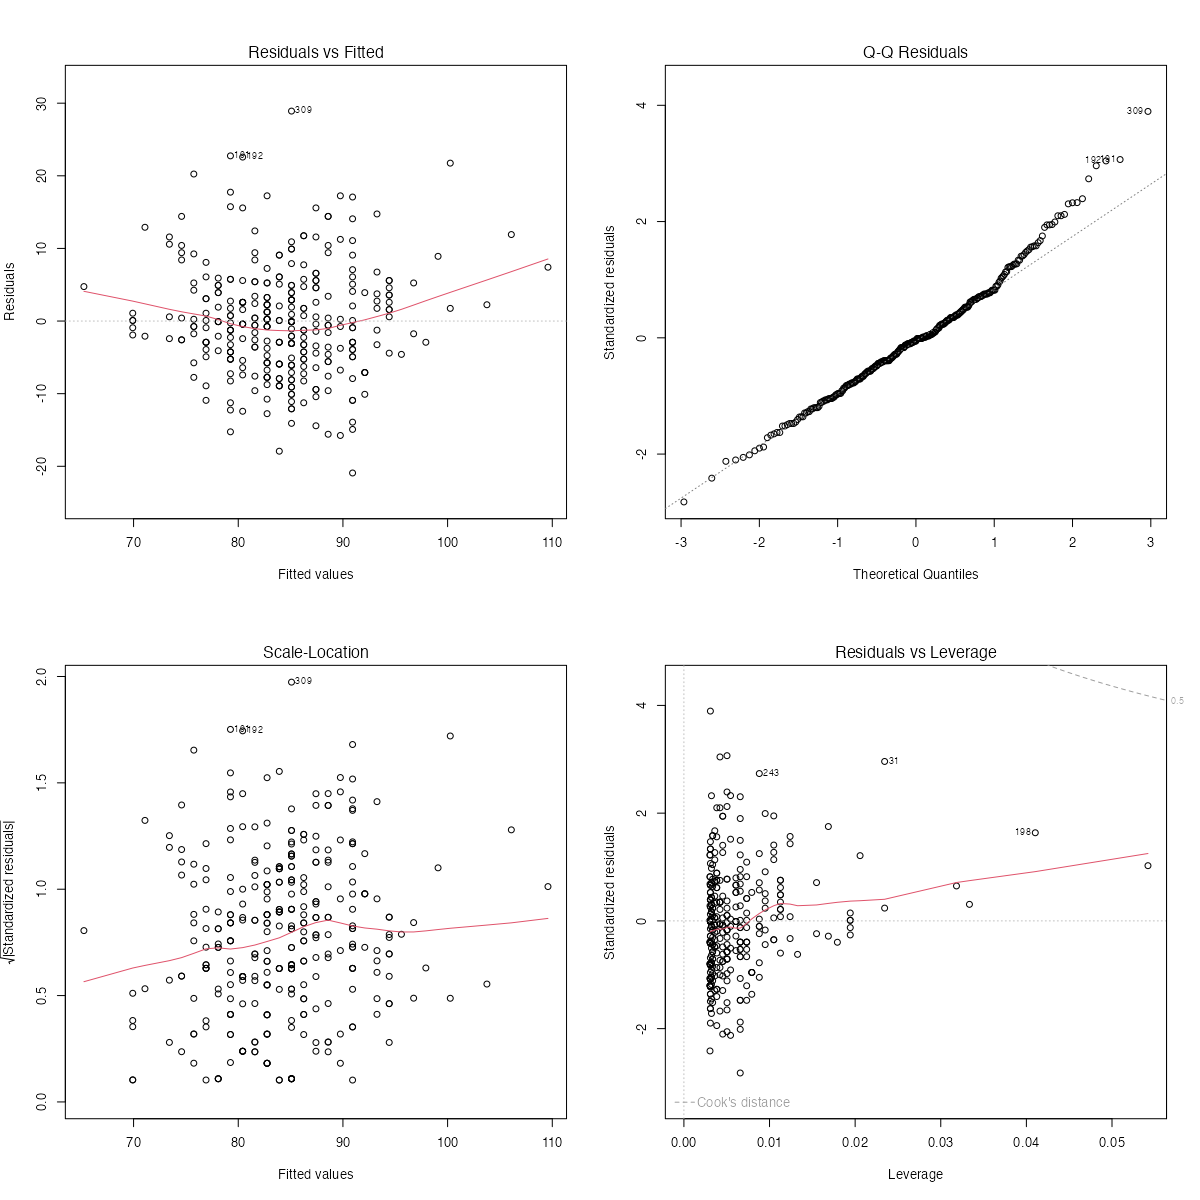
\includegraphics[keepaspectratio,width=0.8\linewidth]{figures/24_linear_model/Rplot_regression.png}
\end{figure}

最初の図(図\ref{fig:24_03}左上)は，残差と予測値の散布図です。回帰分析において，残差$e_i$と予測値$\hat{y}_i$の相関は理論的にゼロになります。実際にそのようになっているかを確認するための図が表示されています。今回の散布図をみると，一定の関係はなさそう(緩やかなU字で，特定の関係があるように思えない)ですね。残差は規則性を持たず，均一に散らばっているはずです。この図を見てそれを確認しましょう。

第二の図(図\ref{fig:24_03}右上)は\keyterm{Q-Qプロット}{Q-Qぷろっと}{Q-Q plot}と呼ばれるものです。Q-Qプロットとは一般的に，データが仮定された確率分布にしたがっているかどうかを表示するためのもので，今回は横軸に正規分布の理論点を，縦軸に残差をプロットしています。理論通りの分布をしていると，左下から右上への45度線上にプロットされていくはずで，このラインから外れるのは理論分布から外れていることになります。今回は右の方，大きな値のところで少し歪みが生じていますが，ほとんどの点がライン上に載っていますので，まあ正規分布していたと考えられるでしょう。

第三の図(図\ref{fig:24_03}左下)は残差標準偏差と予測値のプロット，第四の図(図\ref{fig:24_03}右下)は残差とレバレッジの散布図です。レバレッジとは，各データ点がモデルに与える影響の大きさの指標です。これらも残差の分布が均一であるか，外れ値がないか，というところを検証するためのものです。

これらの図をみて残差が正規分布という仮定にしたがっているか，ということを確認することが重要です。こうした\keyterm{残差診断}{ざんさしんだん}{residual diagnostics}は，モデルの適合性や仮定の妥当性を評価しておくことが重要です。最尤法は確率モデルなのですから。


\section{線形モデルの拡張}
さて，こうしてみてくると，最小二乗法と最尤法，結局答えが同じになるのに，なぜこんな回りくどい話をするのかと思うかもしれません。大事なのは線形モデルが確率モデルになったというところで，確率モデルになることで適用できる範囲が広がるから，というのが1つの答えです。

線形で現象を記述する，つまり$\hat{y} = \beta_0 + \beta_1 x_1 + \beta_2 x_2 + \cdots$のように，説明変数$x$の線形結合で予測値$\hat{y}$を表現する，という考え方は単純で分かりやすいです。重回帰分析における偏回帰係数は，条件つきの係数として解釈するという注意が必要ですが，ある変数が1単位増加したときに予測値がどれだけ変化するか，という直感的な理解が可能です。

人間や社会を扱う現象がすべて線形で説明できる，ということはあり得ません。勉強すればその時間に応じて成績がぐんぐん伸びる，というようなことは，残念ながら実際にはあまりないことかもしれません。現実的ではないかもしれませんが，俯瞰的に見れば，あるいは平均的に見れば，概ね線形関係があるとか，線形で例えてもいいだろう，というぐらいです。人文社会科学で線形モデルが使われるのは，ある程度の適合度を犠牲にしても，解釈のしやすさを優先するからです。

この線形結合で表したものを\keyterm{線形予測子}{せんけいよそくし}{linear predictor}と呼びます。そして，この予測値を中心に確率分布が広がっている，と考えましょう。そして，ここからが大事なポイントですが，この確率分布は必ずしも正規分布である必要はない，ということです。

たとえばベルヌーイ分布は，0/1の二値データを表現する確率分布でした。ベルヌーイ分布はパラメータ$\theta$ひとつだけ持っており，$\theta=0.5$であれば0と1が出てくる確率は五分五分です。言い換えると，平均的に50\%の確率で1が出る，ということです。他にも確率分布はいろいろありますが，それらの確率分布の平均的なパラメータに，線形結合子を対応させることができれば，線形モデルを使って様々なタイプのデータを説明できるようになります。

このように線形モデルを一般化したものを\keytermsub{一般化線形モデル}{いっぱんかせんけいもでる}{generalized linear model, GLM}{線形モデル}{せんけいもでる}と呼びます。

回帰分析を確率モデルという観点から考えれば，線形予測子＋正規分布の組み合わせであり，正規分布の平均パラメータに線形予測子を当てはめたもの，と理解できます。一般化線形モデルは，線形予測子＋誤差分布，あるいは線形予測子＋確率分布の平均的なパラメータ，と考えることができます。これを使えば，必ずしも正規分布的でないデータに対しても，線形的な理解ができるようになります。そして，その時のパラメータの推定方法の一つが最尤法なのです。
\subsection{確率分布としての線形モデル}
\label{thinkWithDistribution}
さてここで，要因計画は線形モデルだという話を思い出してください。そして線形モデルのパラメータを最尤法で推定する，というここでの話を組み合わせましょう。つまり，要因計画のデータ生成メカニズム，確率モデルを考えてみようということです。

要因計画がどのようなものであれ，データの散らばりを生んでいるのは効果，個人差，偶然誤差によるものだと考えるのでした。逆に言えば，これらがなければすべての値は同じになるはずだ，という観点から逆算し，効果，個人差，偶然誤差の大きさを見積もっていったのでした。

ここで，誤差を考える時には確率の考え方を利用してそれをコントロールする，という話を思い出してください。ガウスが考えた誤差論は，平均が$0$，分散$\sigma^2$で散らばる正規分布に従うのでした。すなわち誤差を$\varepsilon_{i}$とすると，次のように表現できます。
\begin{align}
\varepsilon_{i} \sim N(0, \sigma)
\end{align}


群間計画の場合は，各観測値$y_i$を切片$\beta_0$と効果$\beta_1$と誤差に分けます。$X_i$は，統制群なら$0$，実験群なら$1$をとる変数です。
\begin{align}
y_i = \beta_0 + \beta_1 X_i + \varepsilon_i
\end{align}
\begin{align}
\varepsilon_i \sim N(0, \sigma)
\end{align}

イメージでいうなら次のような形です。
\begin{figure}[h]
	\centering
	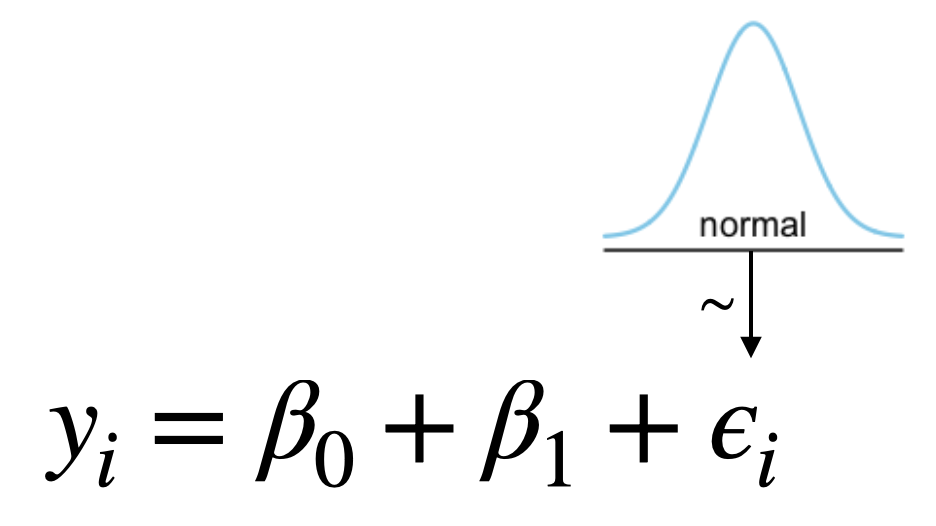
\includegraphics[keepaspectratio,width=0.45\linewidth]{figures/21_Within/between_eq.png}
\end{figure}

$\varepsilon_i$が正規分布に従うのですが，$\beta_0+\beta_1 X_i$のところは確率的に変わるものではないことに注意してください。ここが確率的に変わらないということをよく考えれば，数式に沿ってある値が足されることと同じです。確率分布にある数字を加えると，その分布の位置がずれますね。正規分布は位置と幅でその特徴が作られているのですが，右辺全体で見ると，$\beta_0+\beta_1 X_i$のところは，正規分布の位置をずらすことでもあります。

ずれた分布は，正規分布の平均値が$\beta_0+\beta_1 X_i$ですから，式全体を整えると次のようになります。

\begin{align}
y_i \sim N(\beta_0+\beta_1 X_i , \sigma)
\end{align}

この式のポイントは，$y=$ではなく$y\sim$になっているところです。データが正規分布に従う，という形に変わったのです。線形モデル(要因計画)はこのように，\textbf{確率分布の位置パラメータに数式(モデル)を当てはめる}こととも言えます。

さらにさらに。
群内計画の場合は，個人差$\delta_i$も計算できるのでした。この個人差というのも，たくさん集めると確率的な傾向を表してくるはずで，とくに個々人の生得的な性質に関係するのであれば，それはまた正規分布に従うと言えるでしょう。個人差は全体平均からのずれとして捉えるので，その平均は$0$と置きます(平均を$\psi$\footnote{$\psi$はギリシア文字でプサイと読みます。大文字は$\Psi$であり，心理学Psychologyをギリシア語で表現した最初の文字になります。}のような記号で置くこともできますが，切片$\beta_0$と区別がつかないので$0$とします)。これを踏まえて表現すると次のようになります。
\begin{align}
\delta_i \sim N(0 , \tau)
\end{align}

さてそうすると，群内計画の場合は2つの異なる正規分布が混ぜ合わさった形になっていることになります。式で書くと次のようになりますね。
\begin{align}
y_{ij} = \beta_0 + \delta_i + \beta_j X_{ij} + \varepsilon_{ij}
\end{align}
\begin{align}
\delta_i \sim N(0,\tau), \quad \varepsilon_{ij} \sim N(0,\sigma)
\end{align}

この式をイメージで表すと，次のような形になります。
\begin{figure}[h]
	\centering
	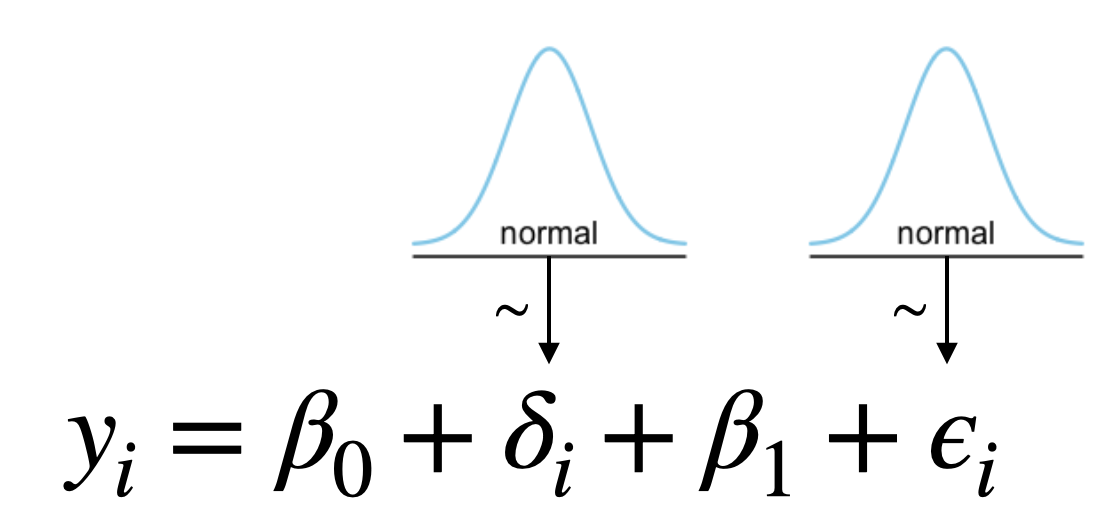
\includegraphics[keepaspectratio,width=0.45\linewidth]{figures/21_Within/within_eq.png}
\end{figure}

このように確率をふまえたモデルで考えると，群内計画のデータには，全員に共通の効果(固定効果)と，個人ごとに確率的に変わる効果(変量効果)の両方が含まれていることになりますから，\keyterm{混合効果モデル}{こんごうこうかもでる}{mixed effect model}と呼ぶことがあります。先ほどの群間計画では，$\beta_0+\beta_1 X_i$で平均値をずらした正規分布にデータが従うことになりましたが，群内計画では$\beta_0+\beta_1+\delta_i$がすでに確率的に分布し，それが平均値となった確率分布がデータの従う分布になる，つまり(誤差の)正規分布の中に(個人差の)正規分布が入れ子になった形でモデルが表現されたことになります。全員に共通の効果(固定効果)と，個人ごとに確率的に変わる効果(変量効果)が混ざっているので，\textbf{混合}というのですね。先ほどのデータを使って図で表現するなら，図\ref{fig:24_04}のようになります。
\begin{figure}[h]
    \centering
	\caption{混合効果モデルのイメージ}
	\label{fig:24_04}
    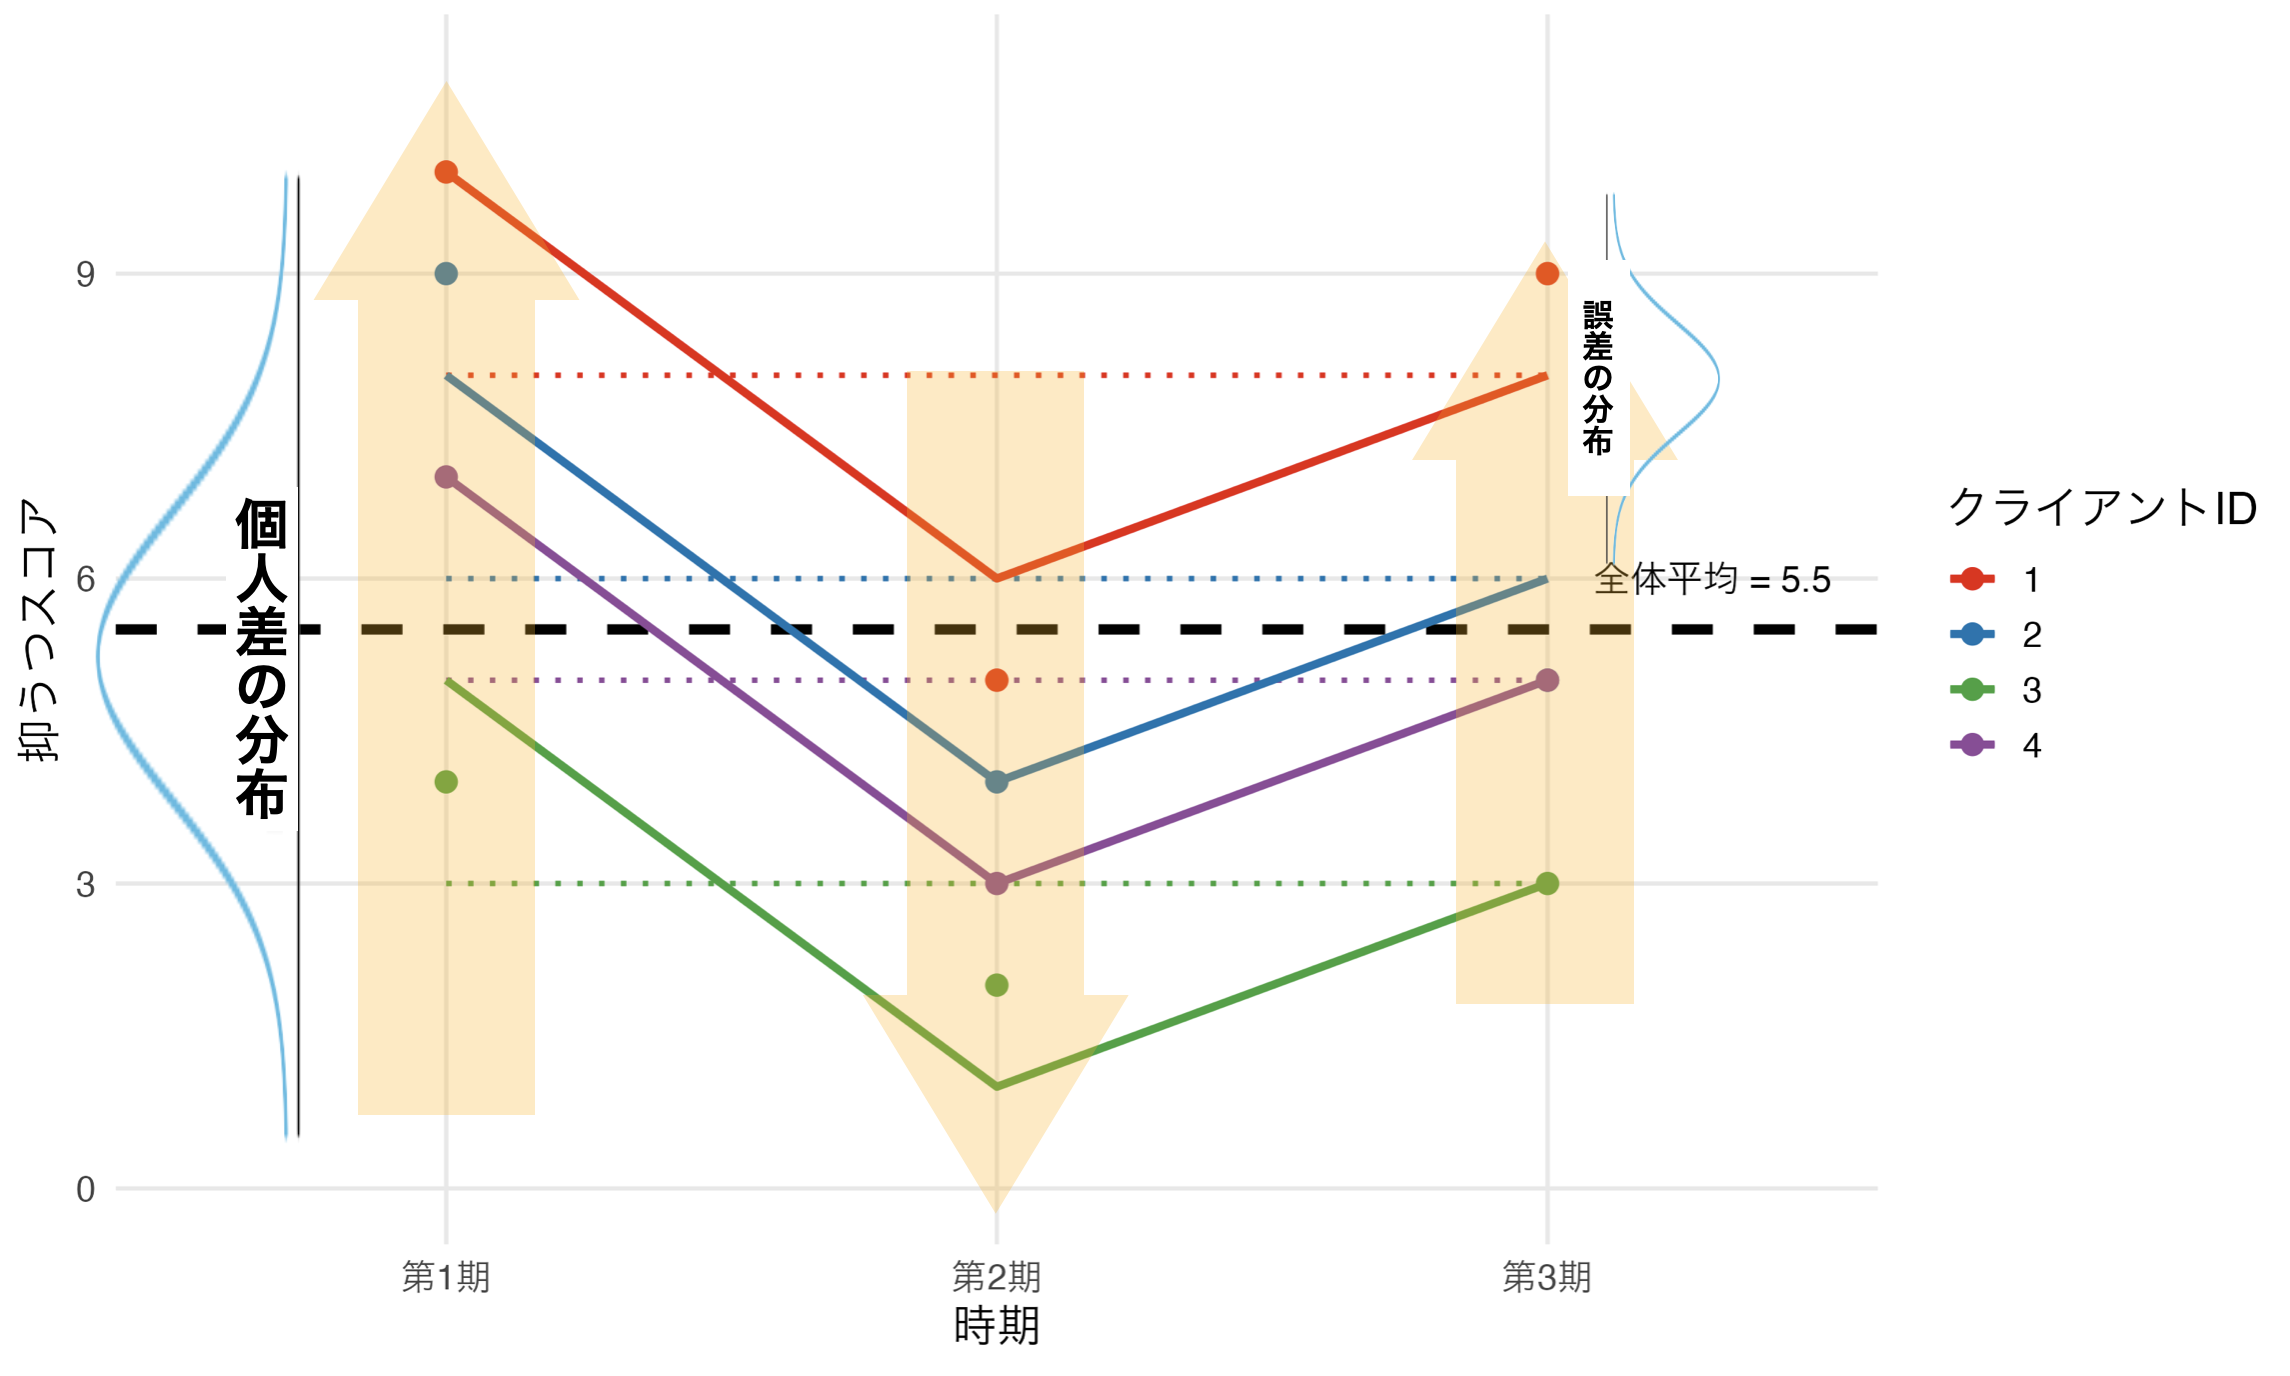
\includegraphics[keepaspectratio,width=0.85\linewidth]{figures/21_Within/mixed_model.png}
\end{figure}

図で表すとかえってわかりにくくなったかもしれませんが，ポイントは，群内計画では個人差も確率的に変化する要素として捉えられる，ということです。さらに言えば，確率的な要素として考えるということは各個体・各実現値ひとつひとつの個性を考えるのではなく，それらは相互に交換可能な偶然の要素であり，全体的な傾向にしたがっていると考えることでもあります。

今回は個人差の要素として考えましたが，実験計画では「等価な刺激」を複数用意して，それらをランダムに割り当てる，ということもよく行います。たとえば記憶の実験として，無意味綴りの単語を覚えてもらって，幾つ覚えられたかを調べる，ということを考えます。実験参加者は「めぬそ」「きたへ」など，全く意味のない単語を覚えるわけですが，全員が同じものを同じ順番で覚える必要はありません。三文字のひらがなで意味を成さない組み合わせ，という条件を満たす単語を複数用意し，それらをランダムに割り当てることで，刺激の個性を抑え，実験参加者の個性も抑えることができます。このような場合も，刺激の個性は確率的に変化する要素として捉えられるわけです。この刺激グループの各要素が持つ個性も，個人差と同じように正規分布に従うと考えられますから，混合効果モデルとして扱います。

このように個人差も刺激の個性も，さらには実験を行う日や場所なども，確率的に変化する要素として捉えられるわけです。これらすべてを混合効果モデルとして扱うことも可能であり，実際にそういう分析手法も存在します(線形混合モデル，Linear Mixed Modelなど)。たとえば同じ実験を複数の国や地域，実験室で行ったものを統合した\keyterm{メタ分析}{めたぶんせき}{meta analysis}などでは，実験室ごとの違いも確率的に変化する要素として捉え，混合効果モデルで分析することがあります。

もっともっと面白いことを言えば，係数$\beta$も確率的に変化する要素として捉えることもできます。いろいろな効果の現れ方が，個人や集団，実験室ごと，あるいは地域や国ごとに少しずつ異なるということも考えられるでしょう。もちろん全体的な効果はありますが，それに加えてローカルな影響があり，それが切片だけでなく傾きにも現れているかもしれません。このように考えるモデルは\keytermsub{階層線形モデル}{かいそうせんけいもでる}{hierarchical linear model}{線形モデル}{せんけいもでる}などと呼ばれ，ベイズ統計学の枠組みで扱われることが多いです。ここでは詳細には立ち入りませんが，実験計画法の理論がこのように発展していることを知っておいてください。


\section{一般化線形モデル}
一般化線形モデルは，線形予測子と確率分布のセットで考えるということでした。
しかし，ここで注意が必要です。線形予測子は$\eta = \beta_0 + \beta_1 x_1 + \beta_2 x_2 + \cdots$のように表されますが，この値は原理的にはどのような値にもなり得ます。正の値でも負の値でもいいですし，ものすごく大きな数字や小さな数字になることもあるでしょう。

ところで，たとえば確率分布として先ほどのベルヌーイ分布を考えたとしましょう。ここで線形予測子を当てはめるのはパラメータ$\theta$ですが，これは表が出る確率を表すパラメータですから，$0 \leq \theta \leq 1$という制約があります。線形予測子はどんな値にもなり得るので，そのまま当てはめるとこの範囲を超えてしまいます。

そこで，線形予測子$\eta$と，確率分布の平均的なパラメータ$\mu$(ベルヌーイ分布なら$\theta$)を結びつける関数を用意します。パラメータから線形予測子への変換$g(\mu) = \eta$を\keyterm{リンク関数}{りんくかんすう}{link function}とよび，その逆の線形予測子からパラメータへの変換$g^{-1}(\eta) = \mu$を\keyterm{逆リンク関数}{ぎゃくりんくかんすう}{inverse link function}と呼びます。用語がややこしいですが，リンク関数はデータの中心傾向を表すパラメータを，線形予測子の尺度へ写す関数であると考えてください。これに対し，私たちは線形予測子でデータがどう変わるか，という解釈をしたいわけです。つまり中心傾向を表す値に線形予測子を当てはめたいわけですから，リンクの逆の作用をする計算が必要です。そこでこれを逆リンク関数と呼びます。いうまでもないことですが，逆リンク関数の逆はリンク関数です。

たとえば，ベルヌーイ分布のパラメータ$\theta$に線形予測子を当てはめるときには，逆リンク関数としてロジスティック関数を用います。ロジスティック関数は，次のように表されます。
\begin{align}
\theta = \frac{1}{1 + \exp(-\eta)}
\end{align}

この関数は，線形予測子$\eta$がどんな値であっても，出力が$0$から$1$の範囲に収まるようになっています(図\ref{fig:24_05})。なお，この逆がリンク関数で，ロジット関数$\eta = \log\frac{\theta}{1-\theta}$になります。

\begin{figure}[ht]
	\centering
	\caption{ロジスティック関数：線形予測子$\eta$がどのような値をとっても，出力$\theta$は0から1の範囲に収まる}
	\label{fig:24_05}
	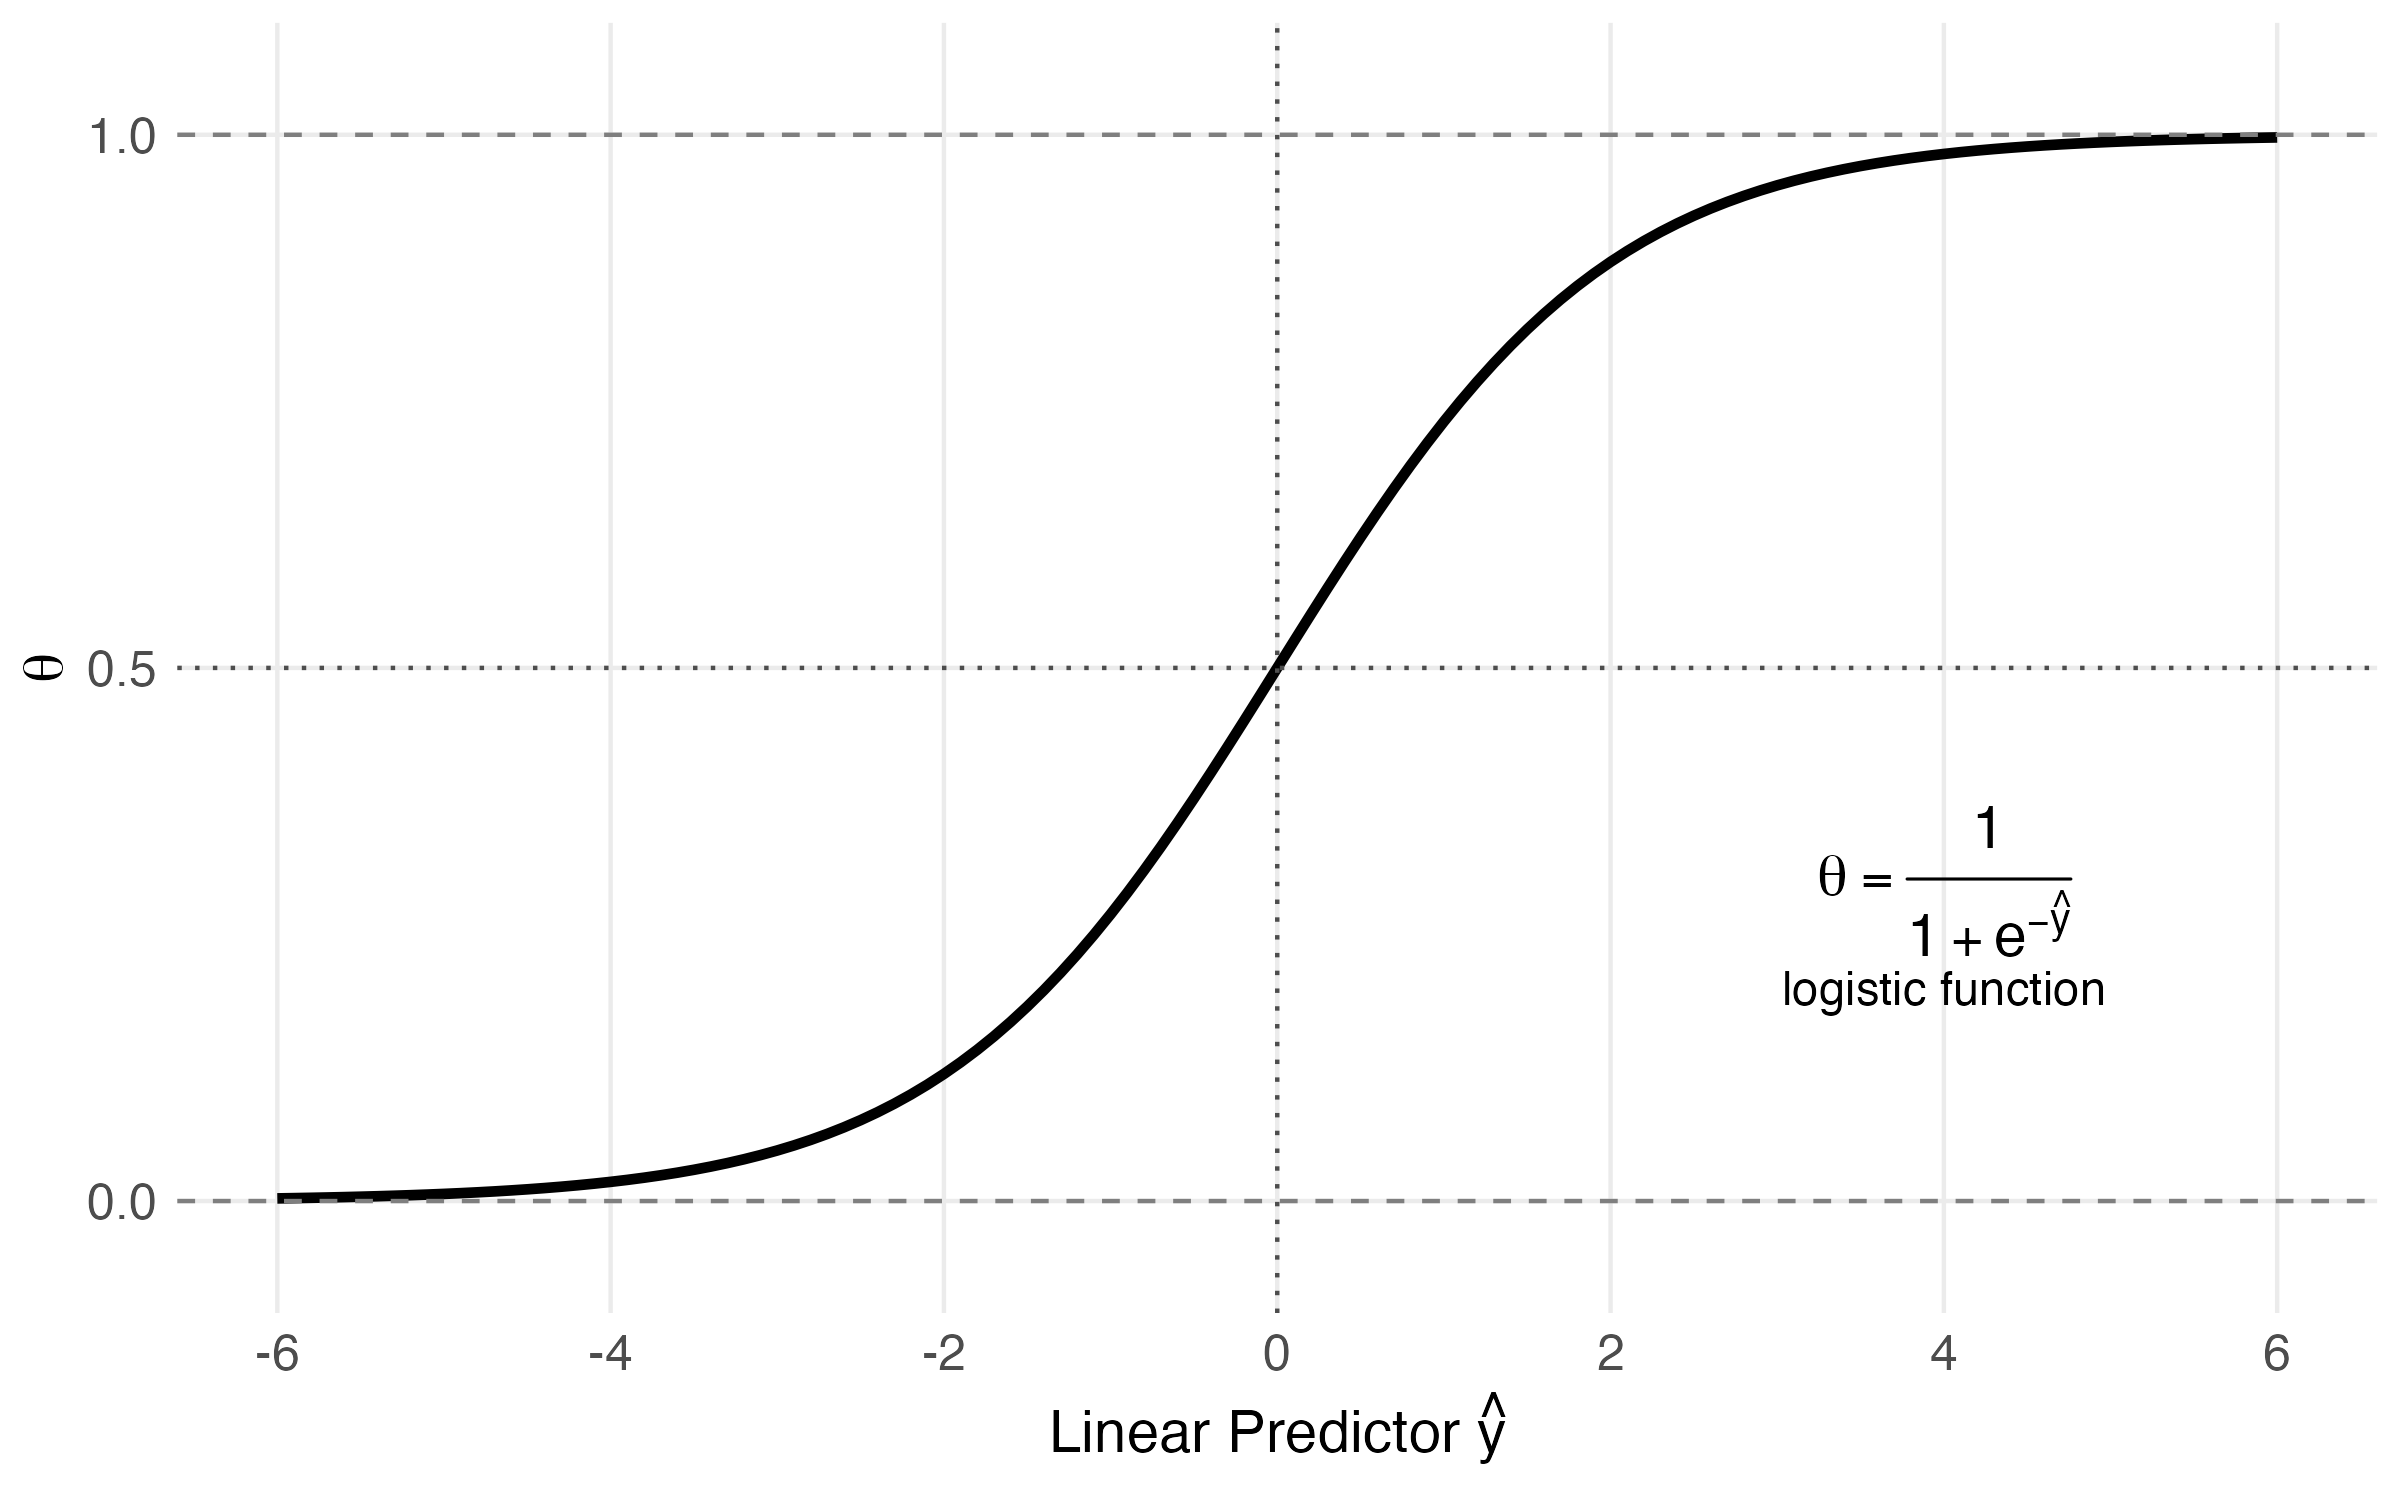
\includegraphics[keepaspectratio,width=0.8\linewidth]{figures/24_linear_model/logistic_function.png}
\end{figure}

このように，一般化線形モデルでは，確率分布のパラメータの定義域に応じた適切な(逆)リンク関数を選ぶことで，線形予測子を様々な確率分布と結びつけることができます。正規分布の場合はリンク関数が恒等関数，$y=x$という何の変化もさせない関数になります。参考までに，表\ref{tbl:24_01}に，変数の種類と確率分布・逆リンク関数の対応をまとめました。これらを駆使すると，どんなデータがあっても，一般化線形モデルを当てはめることができますね。

\begin{table}[htb]
\centering
\caption{変数の種類と確率分布・逆リンク関数の対応}
\label{tbl:24_01}
\renewcommand{\arraystretch}{2.5}
\everymath{\displaystyle}
\begin{tabular}{llll}
\hline
変数の種類 & 確率分布 & 逆リンク関数 & 数値の制約 \\
\hline
量的 & $Normal(\mu,\sigma^2)$ & $\mu =  \eta$ & $\mu \in \mathbb{R}$ \\
二値 & $Bernoulli(\mu)$ & $\mu = \frac{1}{1+\exp(-\eta)}$ & $0 \leq \mu \leq 1$ \\
カウント & $Poisson(\mu)$ & $\mu = \exp(\eta)$ & $\mu > 0$ \\
名義 & $Categorical(...,\mu_k,...)$ & $\mu_k = \frac{\exp(\eta_k)}{\sum_j \exp(\eta_j)}$ & $0 \leq \mu_k \leq 1$ \\
順序 & $Categorical(...,\mu_k,...)$ & $\mu_k = \Phi\left(\frac{\theta_k - \eta}{\sigma}\right) - \Phi\left(\frac{\theta_{k-1} - \eta}{\sigma}\right)$ & $0 \leq \mu_k \leq 1$ \\
\hline
\end{tabular}
\end{table}

\section{課題}

\paragraph{回帰モデルの確率表現}
回帰モデル$y_i = \beta_0 + \beta_1 x_i + \varepsilon_i$を確率モデルとして表現したとき，正しい記述はどれですか。
\begin{itemize}
	\item $y_i$は確定的な値であり，確率分布には従わない
	\item 誤差項$\varepsilon_i$が正規分布に従うとき，$y_i$も正規分布に従う
	\item 線形予測子$\beta_0 + \beta_1 x_i$は確率的に変動する
	\item 誤差項の平均は$\beta_0$である
\end{itemize}

\paragraph{誤差項の仮定}
回帰分析において，誤差項$\varepsilon_i$に関する標準的な仮定として，正しいものはどれですか。
\begin{itemize}
	\item 誤差項の平均は1である
	\item 誤差項は一様分布に従う
	\item 誤差項は平均0の正規分布に従う
	\item 誤差項の分散は観測ごとに異なる
\end{itemize}

\paragraph{最尤推定の目的}
回帰分析で使う「最尤推定」の目的として，最も適切なものを一つ選んでください。
\begin{itemize}
	\item データの中から最大値を見つけること
	\item データがモデルから得られる尤もらしさ(尤度)が最も高くなるようにパラメータを推定すること
	\item データの平均値をそのままパラメータの推定値とすること
	\item データの平均値を求めること
\end{itemize}

\paragraph{対数尤度}
最尤推定において，尤度ではなく対数尤度を用いる理由として，最も適切なものはどれですか。
\begin{itemize}
	\item 対数をとると推定値が変わるから
	\item 確率の積が和に変わり，計算が容易になるから
	\item 対数尤度の方が常に大きな値になるから
	\item 対数をとると正規分布になるから
\end{itemize}

\paragraph{最小二乗法との関係}
正規分布を仮定した回帰分析において，最尤推定と最小二乗法の関係について正しい記述はどれですか。
\begin{itemize}
	\item 最尤推定と最小二乗法は常に異なる推定値を与える
	\item 正規分布を仮定した場合，最尤推定値と最小二乗推定値は一致する
	\item 最小二乗法を使うには，誤差が正規分布に従うと仮定しなければならない
	\item 最尤推定は誤差の分散を推定できないが，最小二乗法は推定できる
\end{itemize}

\paragraph{線形予測子}
線形予測子$\eta = \beta_0 + \beta_1 x_1 + \beta_2 x_2 + \cdots$について，正しい記述はどれですか。
\begin{itemize}
	\item 線形予測子の値は必ず0から1の範囲に収まる
	\item 線形予測子は説明変数の線形結合で表される
	\item 線形予測子は確率分布のパラメータそのものである
	\item 線形予測子には切片項を含めてはならない
\end{itemize}

\paragraph{一般化線形モデル}
一般化線形モデル(GLM)について，正しい記述はどれですか。
\begin{itemize}
	\item 一般化線形モデルは正規分布のみを扱うことができる
	\item 一般化線形モデルでは，線形予測子と確率分布をリンク関数で結びつける
	\item 一般化線形モデルは，リンク関数を使わずに非線形な関係を直接モデル化する
	\item 一般化線形モデルでは最尤推定を使うことができない
\end{itemize}

\paragraph{リンク関数と逆リンク関数}
リンク関数$g(\mu) = \eta$と逆リンク関数$g^{-1}(\eta) = \mu$について，正しい記述はどれですか。
\begin{itemize}
	\item リンク関数は線形予測子をパラメータに変換する
	\item 逆リンク関数は線形予測子をパラメータに変換する
	\item リンク関数と逆リンク関数は同じものである
	\item 正規分布の場合，リンク関数は対数関数である
\end{itemize}

\paragraph{ロジスティック関数}
ベルヌーイ分布に対する逆リンク関数であるロジスティック関数$\theta = \frac{1}{1+\exp(-\eta)}$について，正しい記述はどれですか。
\begin{itemize}
	\item 線形予測子$\eta$がどんな値でも，出力$\theta$は0から1の範囲に収まる
	\item 線形予測子$\eta$が0のとき，$\theta$は0になる
	\item ロジスティック関数の逆関数は指数関数である
	\item ロジスティック関数はカウントデータに用いる
\end{itemize}

\paragraph{確率分布の選択}
以下のデータの種類と，それに適した確率分布の組み合わせとして，正しいものはどれですか。
\begin{itemize}
	\item 量的データ(連続値) --- ベルヌーイ分布
	\item 二値データ(0/1) --- ポアソン分布
	\item カウントデータ(度数) --- ポアソン分布
	\item 順序データ --- 正規分布
\end{itemize}

\end{document}
